The first graphical interface which the user will see when pressing the button is depicted in Figure \ref{fig::UIProjectCase}
\begin{figure}[ht!]
    \centering
    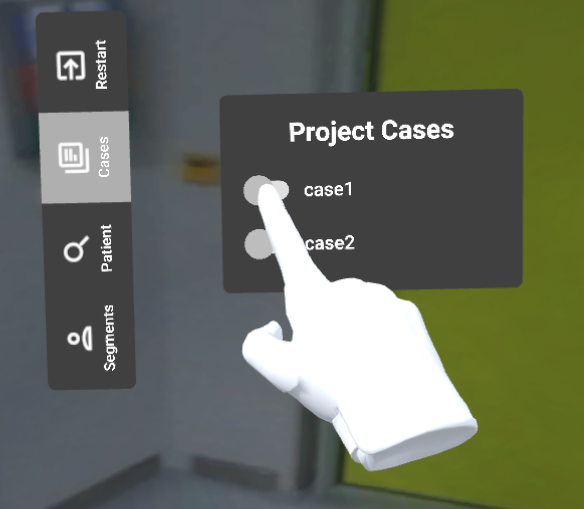
\includegraphics[width=225px]{images/implementation/user_interface/project_cases.png}
    \caption{\label{fig::UIProjectCase}User Interface for the Selection of Project Cases}
\end{figure}
The buttons for loading a case are created dynamically and depend on the number of project case JSON files found in the specified folder.
As will be explained later, the evaluation consists of five distinct scenarios in which distinct procedures have to be performed via the available tools.
By pressing the button by selecting it with the representation of the users hand in the virtual operating room, the project case will be loaded and the patient and information written down in the project case will be display from within the virtual operting room.
On the left side, different submenus can be selected.
Visualization tools can be selected via clicking on 'patient'.
As depicted in Figure \ref{fig::UIPatient}.
Here, tools which are the same for any project case can be used for visualization purposes.
Users have the option to scale the patient, look at the unprocessed patient for comparison and the ability to explode the 3D-Model to help with visualization.
Project cases can also be saved from this menu (Figure \ref{fig::UIPatient}).

\begin{figure}[ht!]
    \centering
    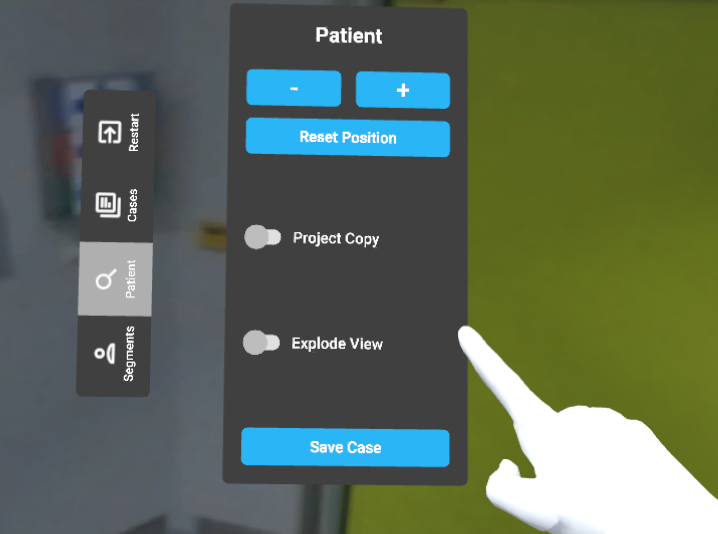
\includegraphics[width=225px]{images/implementation/user_interface/patient.png}
    \caption{\label{fig::UIPatient}User Interface for Patient Visualization Tools}
\end{figure}

\begin{figure}[ht!]
    \centering
    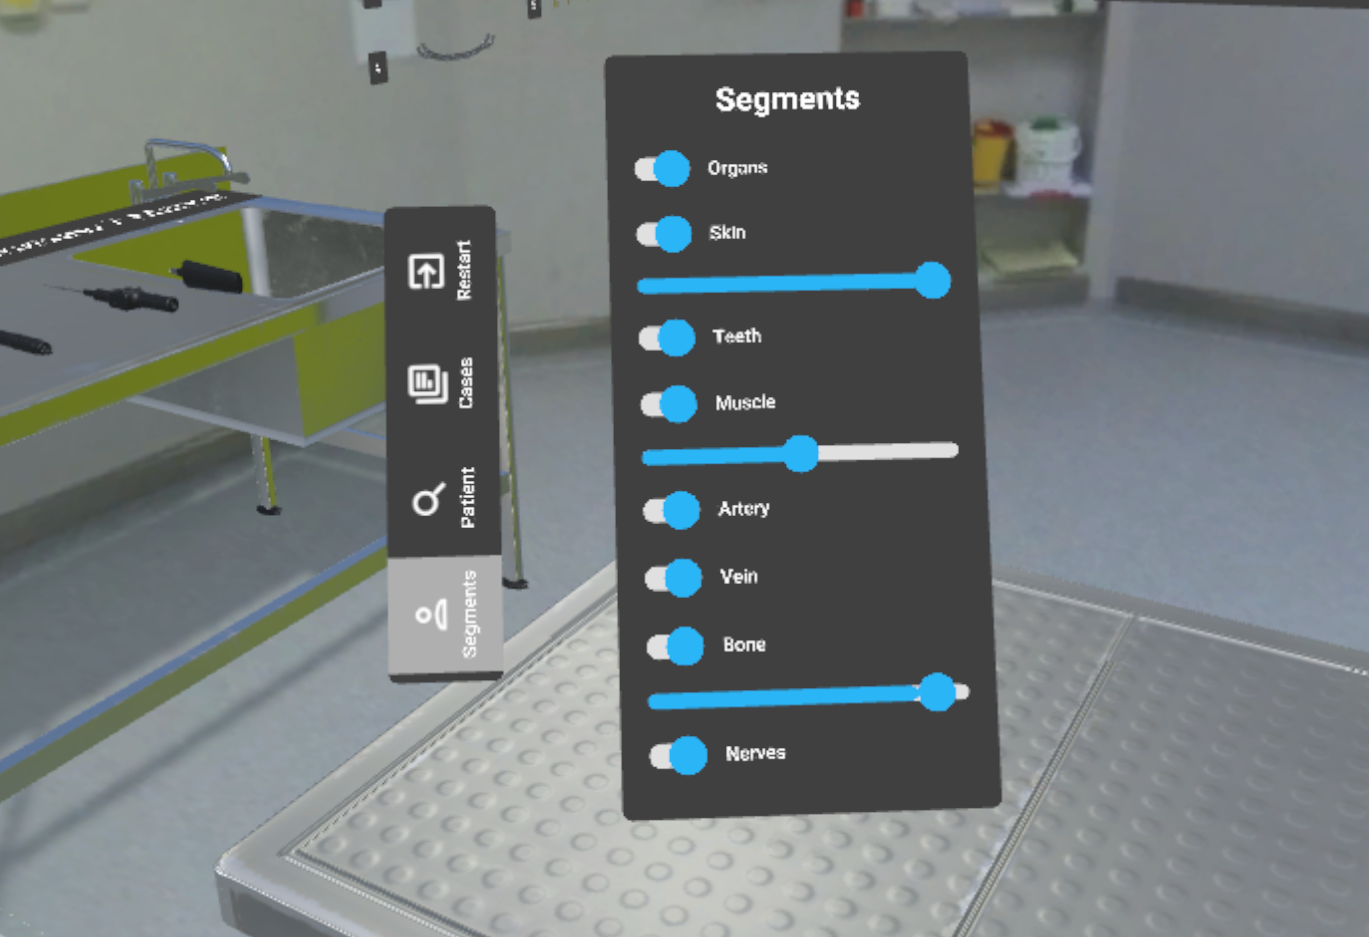
\includegraphics[width=225px]{images/implementation/user_interface/segments.png}
    \caption{\label{fig::UIPatient}User Interface for Patient specific Segments}
\end{figure}
